\documentclass{acm_proc_article-sp}
\usepackage{verbatim}
\usepackage{graphicx}
\begin{document}

\title{Spectral learning for structured partially observable environments}

\numberofauthors{1}

\author{
\alignauthor
Lucas Langer\\
\email{lucas.langer@mail.mcgill.ca}
}

\date{12 August 2015}

\maketitle

\section{Problem and Motivation}

We consider the problem of learning models of time series data in partially observable environments. Typical applications arise in robotics and reinforcement learning with HMMs and POMDPs being the models of choice. We take  interest in environments with structured observations. Standard learning algorithms are not designed to exploit patterns which arise in many practical applications. As a result, we focus on extending a current learning algorithm to exploit such structure. Our approach yields both better predictive accuracy and computational performance when learning smaller models as one does in practice. 

\section{Background and Related Work}

Predictive state representations are used as a model for computing a probability distribution over observations in a dynamical system \cite{littman2001predictive}. There exists a well known spectral algorithm which learns a PSR from empirical data \cite{boots2010closing}. The algorithm makes use of Hankel matrices and singular value decomposition. One can control the number of states in the PSR by only including states with high singular values. The reason for using fewer states is twofold. First, noise in empirical data artificially creates extra states with low singular values. Secondly, reducing the number of states is necessary in practice for computational performance. 

Learning of PSRs began with work on non-spectral methods \cite{DBLP:conf/icml/Wiewiora05}. Spectral algorithms emerged later and became of particular interest because they delivered theoretical guarantees far better than other methods. \cite{boots2010closing}. On the applied side, spectral learning of PSRs has shown promise in planning with timing information \cite{pierrelucplanning2015} and in natural language processing for dependency parsing \cite{balle2013spectral}.

\section{Approach and Uniqueness} 

In our work, we extend the standard PSR learning algorithm by developing a new machinery for performing queries which we call the Base System. The main idea in the Base System is to include transition operators for sequences of observations in addition to those for single observations. We first apply the Base System to predict the time spent by an agent in a stochastic environment. We then progress to systems with multiple observations. Finally, we develop two heuristics: one for choosing operators from data, and another for applying operators in an effective order. The former uses an iterative greedy algorithm while the latter uses a dynamic programming algorithm.

\section{Results and Contributions}

In the experiments that follow, we produce observations by simulating robot motion in stochastic labyrinth environments. The robot explores the labyrinths until it leaves through one of the doors. We compare PSRs learned with the generic algorithm to PSRs learned with different degrees of the Base System. To measure the performance of a PSR, we compare predictions to the actual probability distribution over observations.

\subsection{Double Loops}

In the first experiment we look at the time spent in double loop labyrinths. 

%pasted code to include images]

\begin{figure}[ht!]
\centering

\includegraphics[width=60mm]{lucasplots/monImages/doubleLoopImage.png}
\caption{Double Loop Environment\label{overflow}}
\end{figure}

\begin{figure}[ht!]
\centering
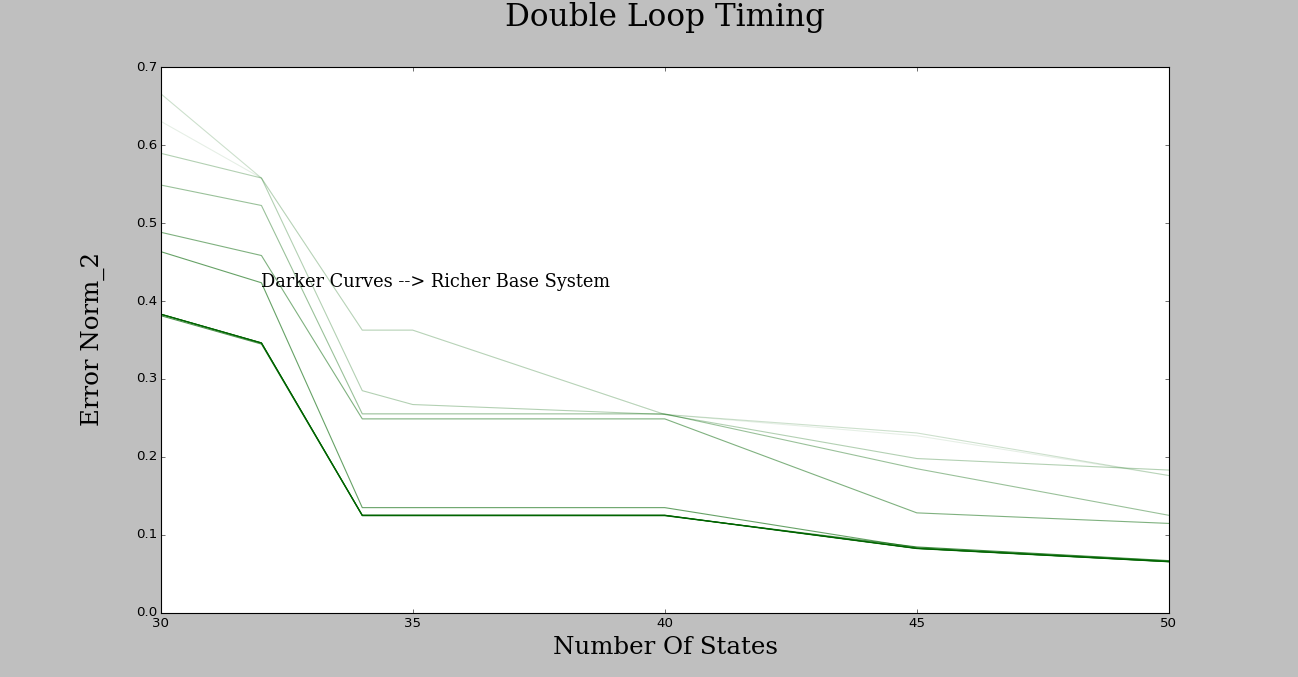
\includegraphics[width=75mm]{lucasplots/monImages/DoubleLoopTiming0.png}
\caption{No Noise in Loops \label{overflow}}
\end{figure}

%ROBOT INSIDE DOULBE LOOP, GET RID OF SYMMETRY
\begin{figure}[ht!]
\centering
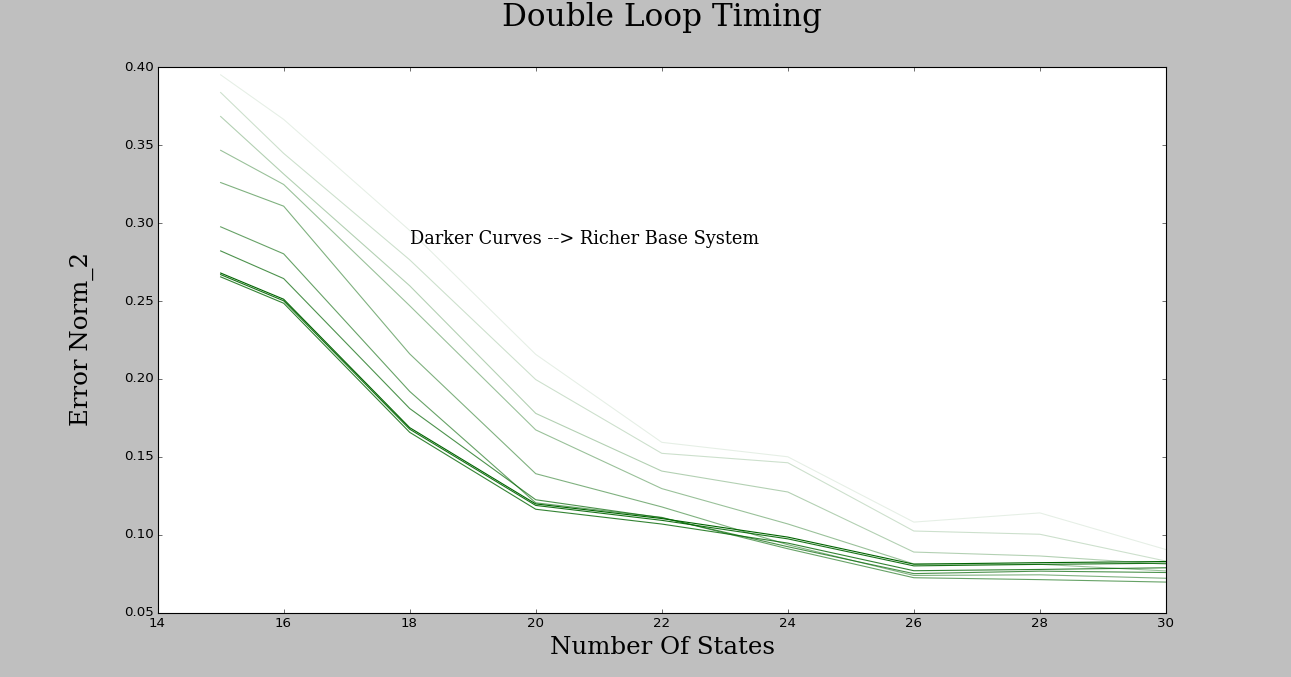
\includegraphics[width=75mm]{lucasplots/monImages/DoubleLoopTiming0_1.png}
\caption{Noise in Loops \label{overflow}}
\end{figure}

The PSR with the Base System significantly lower errors across all model sizes (Figures 2 and 3). In particular, we note that noise in the durations of loops doesn't harm the performance of the Base System.

\subsection{PacMan Labyrinth}

In the second experiment, we look at timing for a PacMan-Type labyrinth. In addition, we use state weightings from the learned PSRs to predict distances between the robot and objects in the environment. 

%\begin{comment}
\begin{figure}[ht!]
\centering
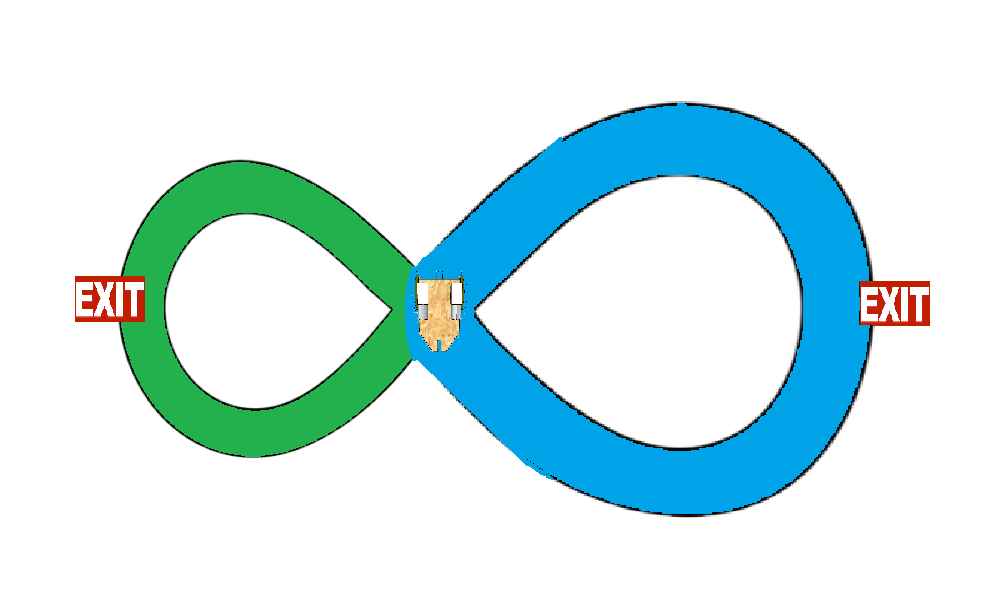
\includegraphics[width=60mm]{lucasplots/monImages/doubleLoopImageMO.png}
\caption{Multiple Observation Environment \label{overflow}}
\end{figure}
%\end{comment}


\begin{figure}[ht!]
\centering
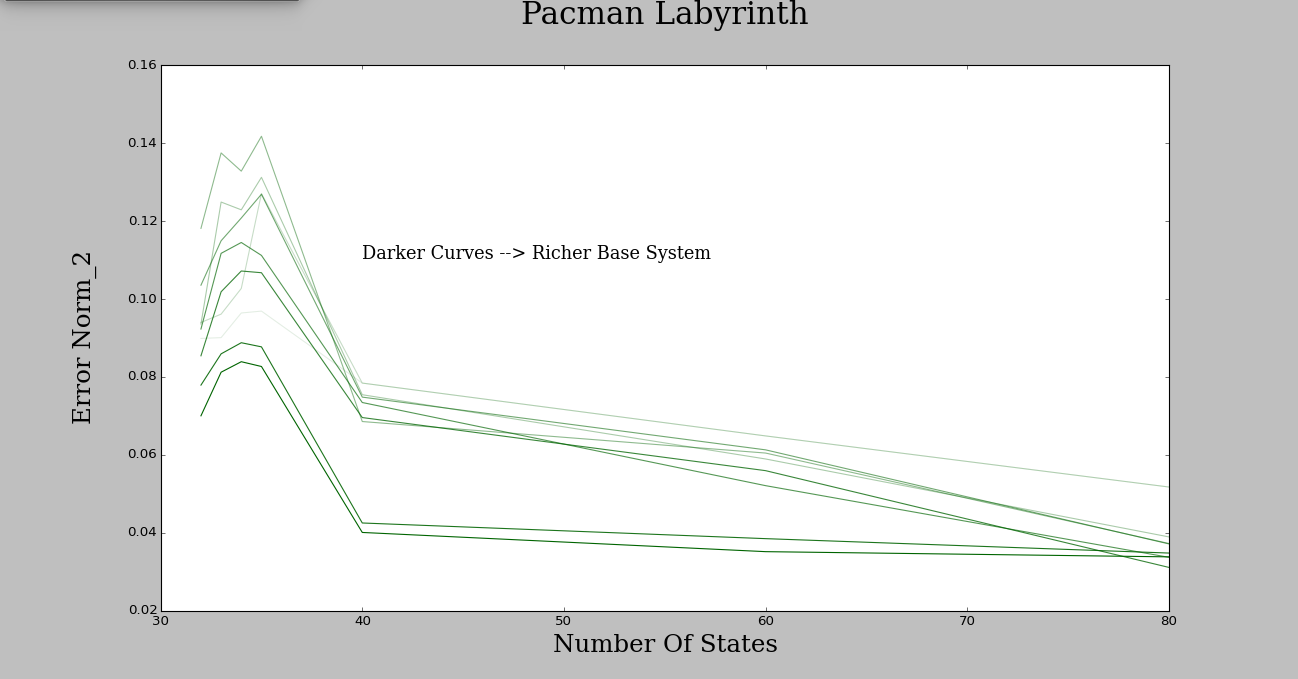
\includegraphics[width=75mm]{lucasplots/monImages/PacmanLabyrinth.png}
\caption{Timing Predictions in Pacman \label{overflow}}
\end{figure}

\begin{figure}[ht!]
\centering
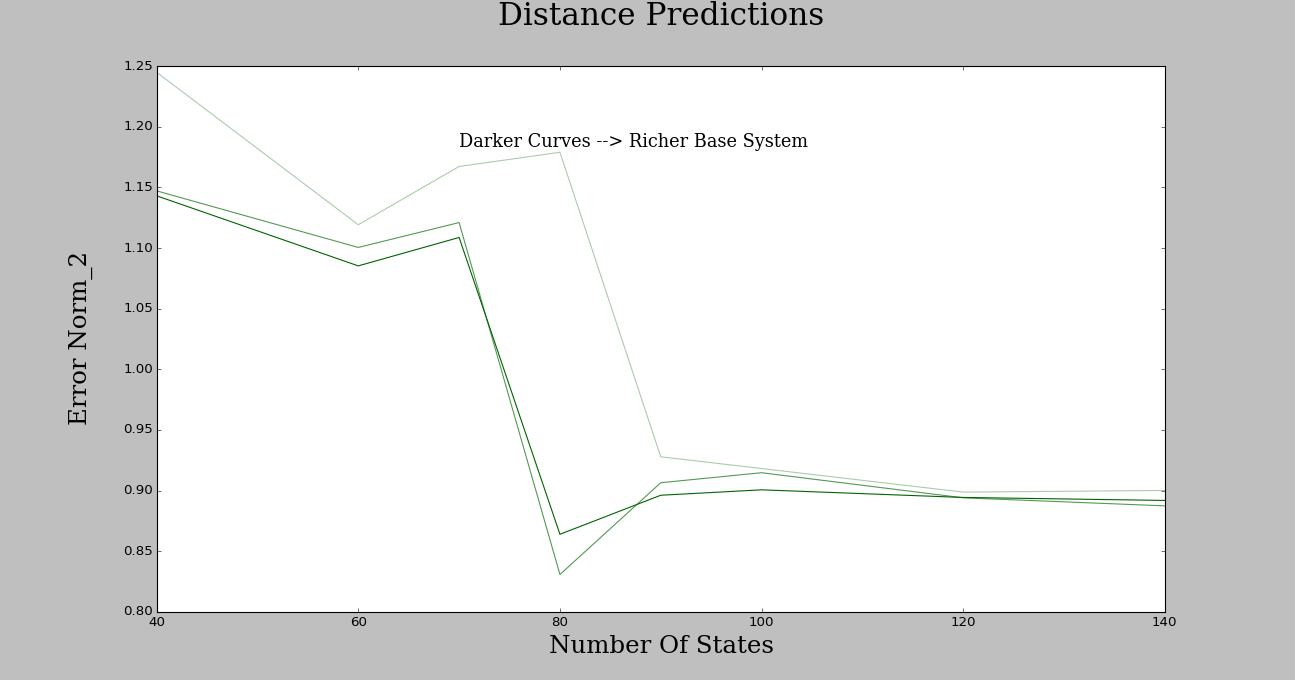
\includegraphics[width=75mm]{lucasplots/monImages/Distance_Predictions.png}
\caption{Distance Predictons\label{overflow}}
\end{figure}

The Base System outperforms the naive PSR for the Pacman environment (Figure 5). It also does better for predicting distances (Figure 6). 

\subsection{Multiple Observations}

Next, we change our set of observations to wall colors of the labyrinth. 

\begin{figure}[ht!]
\centering
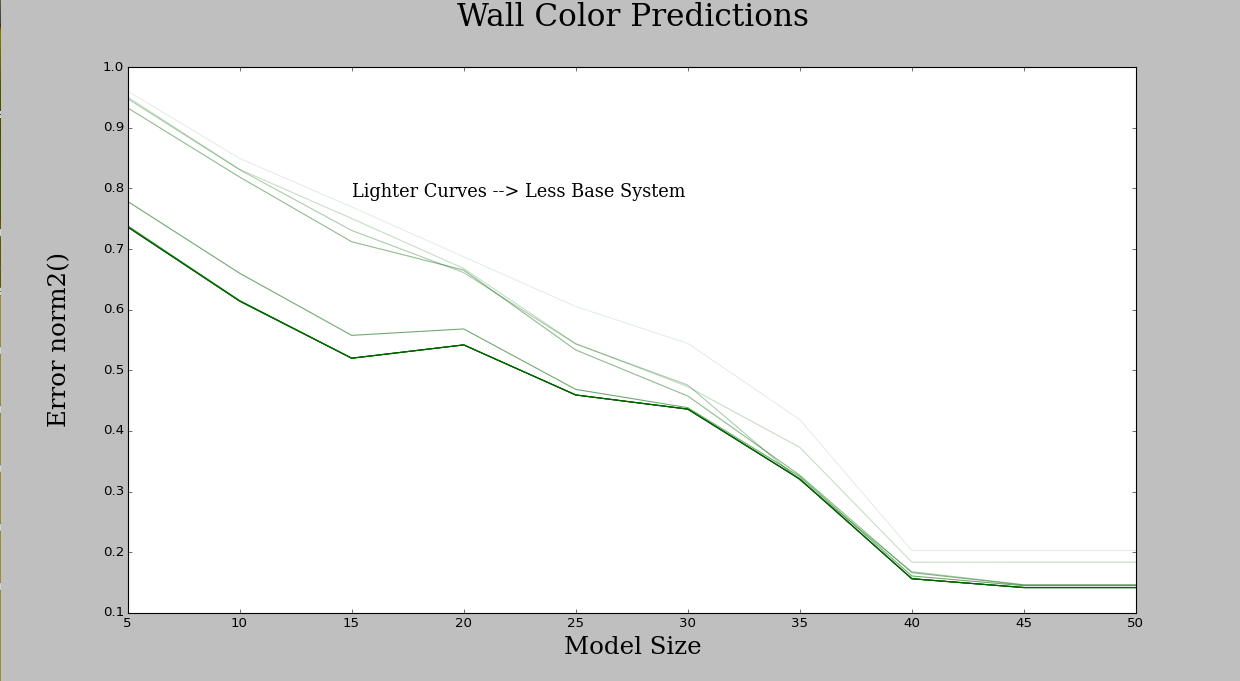
\includegraphics[width=75mm]{lucasplots/monImages/WallColorPredictions.png}
\caption{Predicting Wall Colors \label{overflow}}
\end{figure}

The Base System also does better for loops with multiple observations (Figure 7).

%Cite figures

\section{Relevance and Future Work}
In this work, we showed a way to significantly improve performance of truncated models in applied environments. For future work, we leave a theoretical analysis of the Base System and further optimization of its construction .

%
% The following two commands are all you need in the
% initial runs of your .tex file to
% produce the bibliography for the citations in your paper.
\bibliographystyle{abbrv}
\bibliography{sigproc}  % sigproc.bib is the name of the Bibliography in this case
% You must have a proper ".bib" file
%  and remember to run:
% latex bibtex latex latex
% to resolve all references
%
% ACM needs 'a single self-contained file'!
%.


\end{document}



